%=======================================================
%	PACKAGES AND THEMES
%=======================================================
\documentclass[8pt]{beamer}
\mode<presentation> {
\usepackage{etex}
\usetheme{Boadilla}
\definecolor{navyblue}{rgb}{0.0, 0.0, 0.5}
\definecolor{dkgreen}{rgb}{0,0.6,0}
\definecolor{gray}{RGB}{64, 64, 64}
\definecolor{teal}{RGB}{0, 102, 102}
\definecolor{mauve}{rgb}{0.58,0,0.82}
\usecolortheme[named = navyblue]{structure}
\setbeamercolor{normal text}{fg = gray}
\setbeamercolor{frametitle}{fg = white, bg = navyblue}
\setbeamerfont{framesubtitle}{size = \normalsize}
\setbeamerfont{caption}{size=\footnotesize}
\setbeamercolor{page number in head/foot}{fg = gray}
\setbeamertemplate{footline}%[frame number]
}


\usepackage{graphicx} % Allows including images
\usepackage{booktabs} % Allows the use of \toprule, \midrule and \bottomrule in tables
\usepackage{multicol}
\usepackage[export]{adjustbox}
\usepackage{colortbl}
\usepackage{graphicx} 

\usepackage{tikz}
\usepackage{fancybox}
\usepackage[absolute, overlay]{textpos}
\usepackage{multirow}
\usepackage{siunitx}
\usepackage{tcolorbox}


\usepackage{tikz}
\usepackage{calc}
\newlength{\outerradius}
\newlength{\innerradius}
\setlength{\outerradius}{0.50cm}
\setlength{\innerradius}{0.35cm}

\usepackage{listings}
\lstset{numbers=left,
	numberstyle=\tiny,
	numbersep=5pt,
	breaklines=true,
	showstringspaces=false,
	frame=l ,
	xleftmargin=15pt,
	xrightmargin=15pt,
	basicstyle=\ttfamily\scriptsize,
	stepnumber=1,
	keywordstyle=\color{blue},          % keyword style
  	commentstyle=\color{dkgreen},       % comment style
  	stringstyle=\color{mauve}         % string literal style
}
\lstset{language=R}


%=======================================================
%	TITLE PAGE
%=======================================================

\title{\textbf{Network Definition}}

\author{Dr David Eggleton}

\institute
{
SPRU (Science Policy Research Unit) \\
Business School\\
University of Sussex \\

\medskip

\medskip

\medskip

\includegraphics[width=2.5cm]{../_shared_pics/logo}

\medskip

\textit{{\color{dkgreen}{Week 2}}}\\
}


\date{} % Date, can be changed to a custom date

\begin{document}

\begin{frame}
\titlepage % Print the title page as the first slide

\begin{textblock*}{10pt}(0pt, 0.9\textheight)
\includegraphics[width=4cm]{../_shared_pics/SPRU.png}
\end{textblock*}

\end{frame}


%=======================================================
%	Learning outcomes
%=======================================================

\begin{frame}
\frametitle{Learning Outcomes}

\centering
\footnotesize
\begin{tabular}{lp{5.5cm}l}
\toprule
\multicolumn{2}{l}{\textbf{Learning outcome}} & \textbf{Assessment mode}\\
\hline
\\
\rowcolor{green!20}1 & 
Explain the concept of network and list the main network indicators & 
ESS\\
\\
2 & 
Describe and apply the major techniques for the collection of network data and their statistical analysis & 
ESS, GPN + GWS\\
\\
3 & 
Identify the main characteristics of networks by means of network measures  & 
ESS, GPN + GWS\\
\\
4 &
Employ network analysis techniques to produce network data-based infographics & 
GPN + GWS\\
\\
\bottomrule
\multicolumn{3}{l}{Note: ESS: Essay; GPN: Group Presentation; GWS: Group Written Submission}\\
\end{tabular}

\end{frame}

%------------------------------------------------



%=======================================================
%	Intro slides
%=======================================================

\begin{frame}
\frametitle{Overview}
\tableofcontents[hideallsubsections]
\end{frame}

%------------------------------------------------




%=======================================================
%	Defining a network
%=======================================================
\section{Defining a network}

%------------------------------------------------

\bgroup
\setbeamercolor{background canvas}{bg = navyblue}
\begin{frame}[plain]{}
\begin{center}
\color{white}{\Huge\insertsection}
\end{center}
\end{frame}
\egroup

%------------------------------------------------

\begin{frame}
\frametitle{\insertsection}

From {\color{blue}{natural}} to {\color{blue}{social phenomena}}

\begin{table}
\newcolumntype{C}{>{\centering\arraybackslash} m{.25\textwidth} }
\begin{tabular}{|C|C|C|}
\midrule
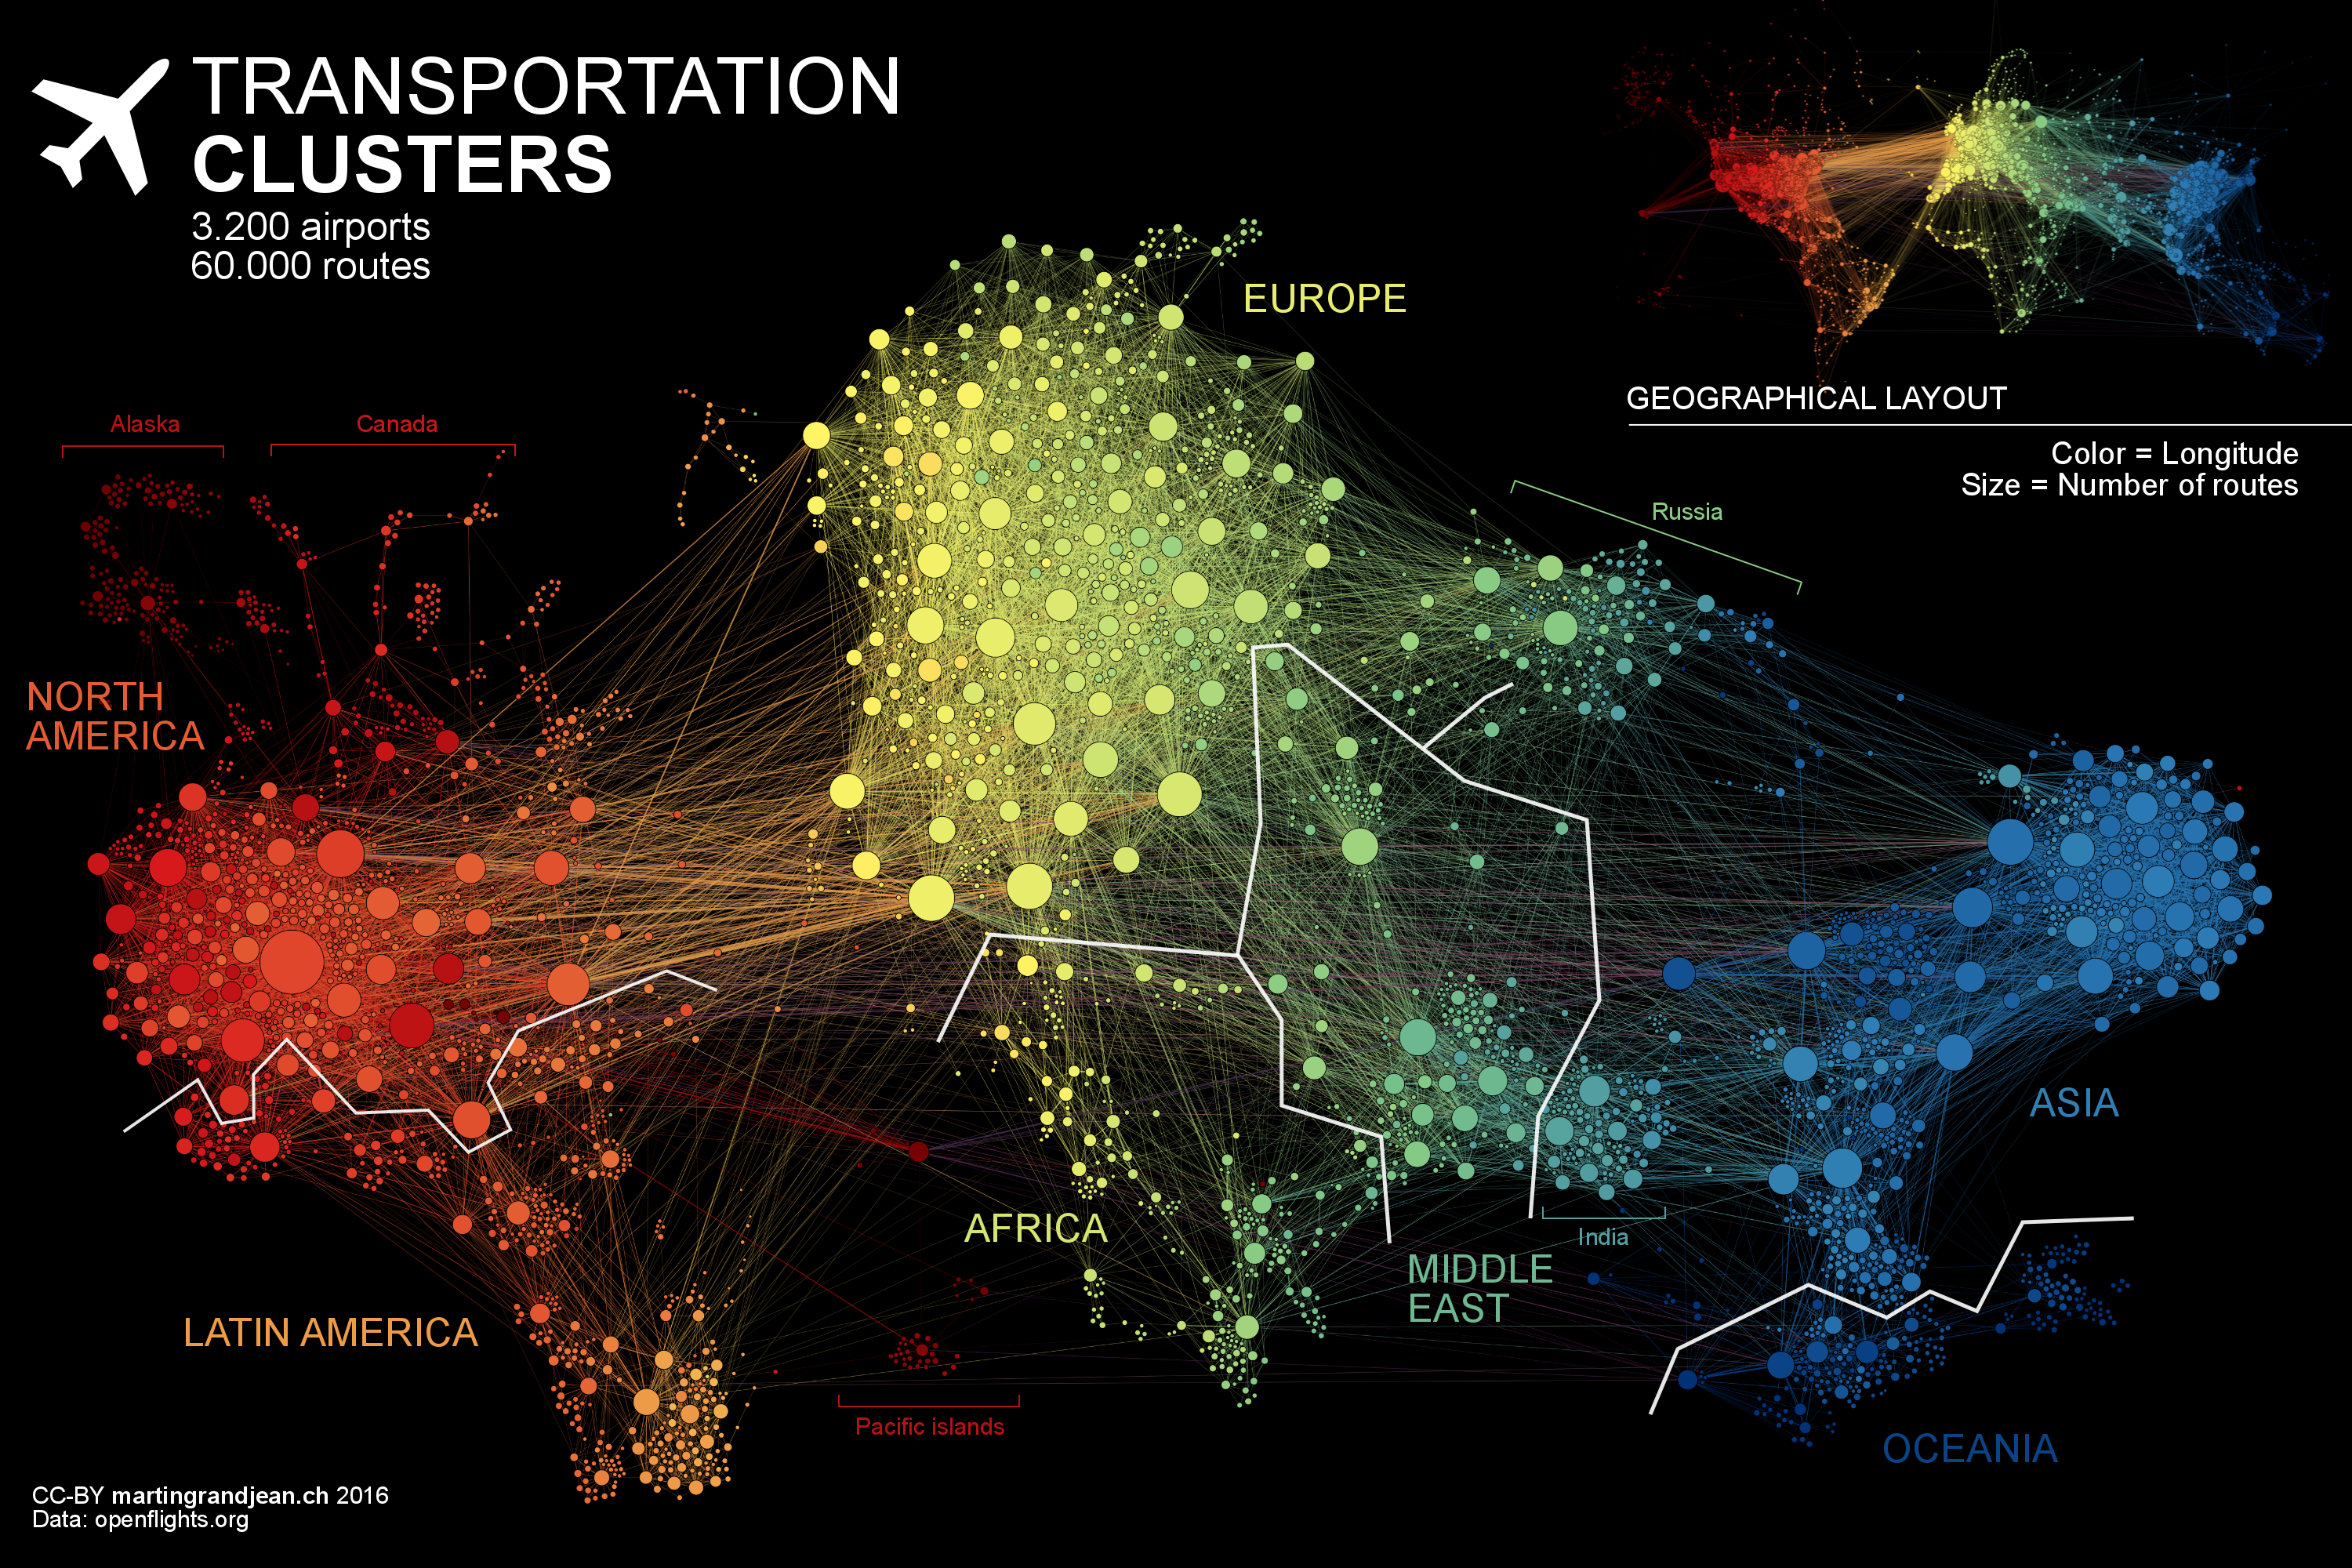
\includegraphics[width=0.25\textwidth, height=0.25\textheight, keepaspectratio]{airports-world-network} &
\includegraphics[width=0.25\textwidth, height=0.25\textheight, keepaspectratio]{facebook} &
\includegraphics[width=0.25\textwidth, height=0.25\textheight, keepaspectratio]{tube} \\
\midrule
\includegraphics[width=0.25\textwidth, height=0.25\textheight, keepaspectratio]{disease_net} &
\includegraphics[width=0.25\textwidth, height=0.25\textheight, keepaspectratio]{crime} &
\includegraphics[width=0.25\textwidth, height=0.25\textheight, keepaspectratio]{outbreak} \\
\midrule
\includegraphics[width=0.25\textwidth, height=0.25\textheight, keepaspectratio]{marvel} &
\includegraphics[width=0.25\textwidth, height=0.25\textheight, keepaspectratio]{nature} &
\includegraphics[width=0.25\textwidth, height=0.25\textheight, keepaspectratio]{open_syllabus} \\
\midrule
\end{tabular}
\end{table}
\end{frame}

%------------------------------------------------

\begin{frame}
\frametitle{\insertsection}
\framesubtitle{Graph theory}


\begin{columns}[c]
\column{.45\textwidth}
We rely on {\color{blue}{graph theory}} to define (social) networks
    \begin{itemize}
    \item Graphs model relations between pairs of objects
    \item Terms and vocabulary to denote structural properties
    \item Formulas to quantify structural properties
    \end{itemize}

\column{.45\textwidth}
\centering
\includegraphics[width=4cm]{graph_theory}\\
\tiny{Source: \cite{Bondy1976}}
\end{columns}

\end{frame}

%------------------------------------------------

\begin{frame}
\frametitle{\insertsection}
\framesubtitle{Graph theory}

\begin{columns}[c]
\column{.45\textwidth} 
	\begin{itemize}
	\item A {\color{blue}{graph}} is defined as: $G(N, E)$
	\item $N$ vertices, $N = {n_1, n_2, ..., n_N}$
	\item $E$ edges, $E = {e_1, e_2, ..., e_E}$
	\item Example: $G(7,8)$
	\end{itemize}

\column{.45\textwidth}
\centering
\includegraphics[width=5cm]{base}
\end{columns}

\end{frame}

%------------------------------------------------

\begin{frame}
\frametitle{\insertsection}
\framesubtitle{Definition}

\centering
\def\arraystretch{1.5}
\begin{tabular}{cc}
\toprule
\textbf{Graph theory} & \textbf{Network science}\\
\hline
Graph & Network\\
Vertex & Node\\
Edge & Link\\
\bottomrule
\end{tabular}

\end{frame}

%------------------------------------------------

\begin{frame}
\frametitle{\insertsection}
\framesubtitle{Graph theory}

\begin{columns}[c]
\column{.45\textwidth} 
	\begin{itemize}
		\item ``A network consists of {\color{blue}{a graph and additional information}} on the vertices or the lines of the graphs'' \cite{deNooy2005}
		\item ``Networks can be conceived as metaphors to visualise {\color{blue}{a (finite) set of edges (links, ties)}} among {\color{blue}{a (finite) set of nodes (vertices)}}'' \cite{Wassermann1994}
	\end{itemize}

\column{.45\textwidth}
\centering
\includegraphics[width=5cm]{base}\\
\end{columns}

\end{frame}

%------------------------------------------------

\begin{frame}
\frametitle{\insertsection}
\framesubtitle{Definition}

\begin{columns}[c]
\column{.45\textwidth} 
{\color{blue}{Nodes}}: entities on which the analysis focuses
	\begin{itemize}
    \item individuals (e.g.\ family members, employees, inventors)
    \item organisations (e.g.\ firms, universities, business units)
    \item documents (e.g.\ publications, patents)
    \item geographical areas (e.g.\ cities, regions, countries)
    \item ...
    \end{itemize}

\column{.45\textwidth}
\centering
\includegraphics[width=5cm]{nodes}
\end{columns}

\end{frame}

%------------------------------------------------

\begin{frame}
\frametitle{\insertsection}
\framesubtitle{Definition}

\begin{columns}[c]
\column{.45\textwidth} 
{\color{blue}{Links (ties)}}: ties linking the entities (modes of interactions)
	\begin{itemize}
    \item formal and informal relations (e.g.\ collaboration, friendship)
    \item biological relations (e.g.\ kinship)
    \item transfer of knowledge and resources (e.g.\ licensing, alliances)
    \item association or affiliation (e.g.\ social club, employer)
    \item physical connections (e.g.\ bridges)
    \item events (e.g.\ sending e-mails, transactions)
    \item ...
    \end{itemize}

\column{.45\textwidth}
\centering
\includegraphics[width=5cm]{base}
\end{columns}

\end{frame}

%------------------------------------------------

\begin{frame}
\frametitle{\insertsection}
\framesubtitle{Example}
\centering
\includegraphics[width=\linewidth,height=0.8\textheight,keepaspectratio]{cpm}\\
\tiny Source: Critical Path Method [\url{www.pmi.org}]
\end{frame}


%NOTE =============
%== Top-left: Earliest start
%== Bottom-left: Latest finish
%== Top-right: Earliest finish
%== Bottom-right: Latest finish
%== Centre: Activity name and duration
%== Links: Dependency between activities
%=================


%------------------------------------------------

\begin{frame}
\frametitle{\insertsection}
\framesubtitle{Example}
\centering
\includegraphics[width=\linewidth,height=0.8\textheight,keepaspectratio]{apple}\\
\tiny Source: Apple's inventor network [\url{http://www.kenedict.com}]
\end{frame}

%NOTE =============
%== Collaboration between inventors
%== Colors represent technological classes
%=================

%------------------------------------------------

\begin{frame}
\frametitle{\insertsection}
\framesubtitle{Example}
\centering
\includegraphics[width=\linewidth,height=0.8\textheight,keepaspectratio]{altruism}\\
\tiny Source: 357 topics from the websites of 125,000 non-profit organizations in the US \cite{Klavans2014}
\end{frame}

%------------------------------------------------

\begin{frame}
\frametitle{\insertsection}
\framesubtitle{Example}

\begin{columns}[c]
\column{.45\textwidth} 
\includegraphics[height=0.4\textheight]{wine1}\\

\column{.45\textwidth}
\centering
\includegraphics[height=0.4\textheight]{wine2}\\
\end{columns}
\medskip
\medskip
\medskip
\centering
\tiny Source: Local knowledge network in 2002 (left) 2006 (right) \cite{Giuliani2013}
\end{frame}

%NOTE =============
%== Wine cluster in Chile and formation of new knowledge ties between wine producers
%=================

%------------------------------------------------

\begin{frame}
\frametitle{\insertsection}
\framesubtitle{Example}
\centering
\includegraphics[width=\linewidth,height=0.8\textheight,keepaspectratio]{mp}\\
\tiny Source: 2015 network of MPs based on Twitter links (\url{www.nesta.org.uk/blog/twitter-network-uk-mps/})
\end{frame}

%NOTE =============
%== A link between two MP is establish if they follow each other.
%=================
%------------------------------------------------

\begin{frame}
\frametitle{\insertsection}
\framesubtitle{Example}
\centering
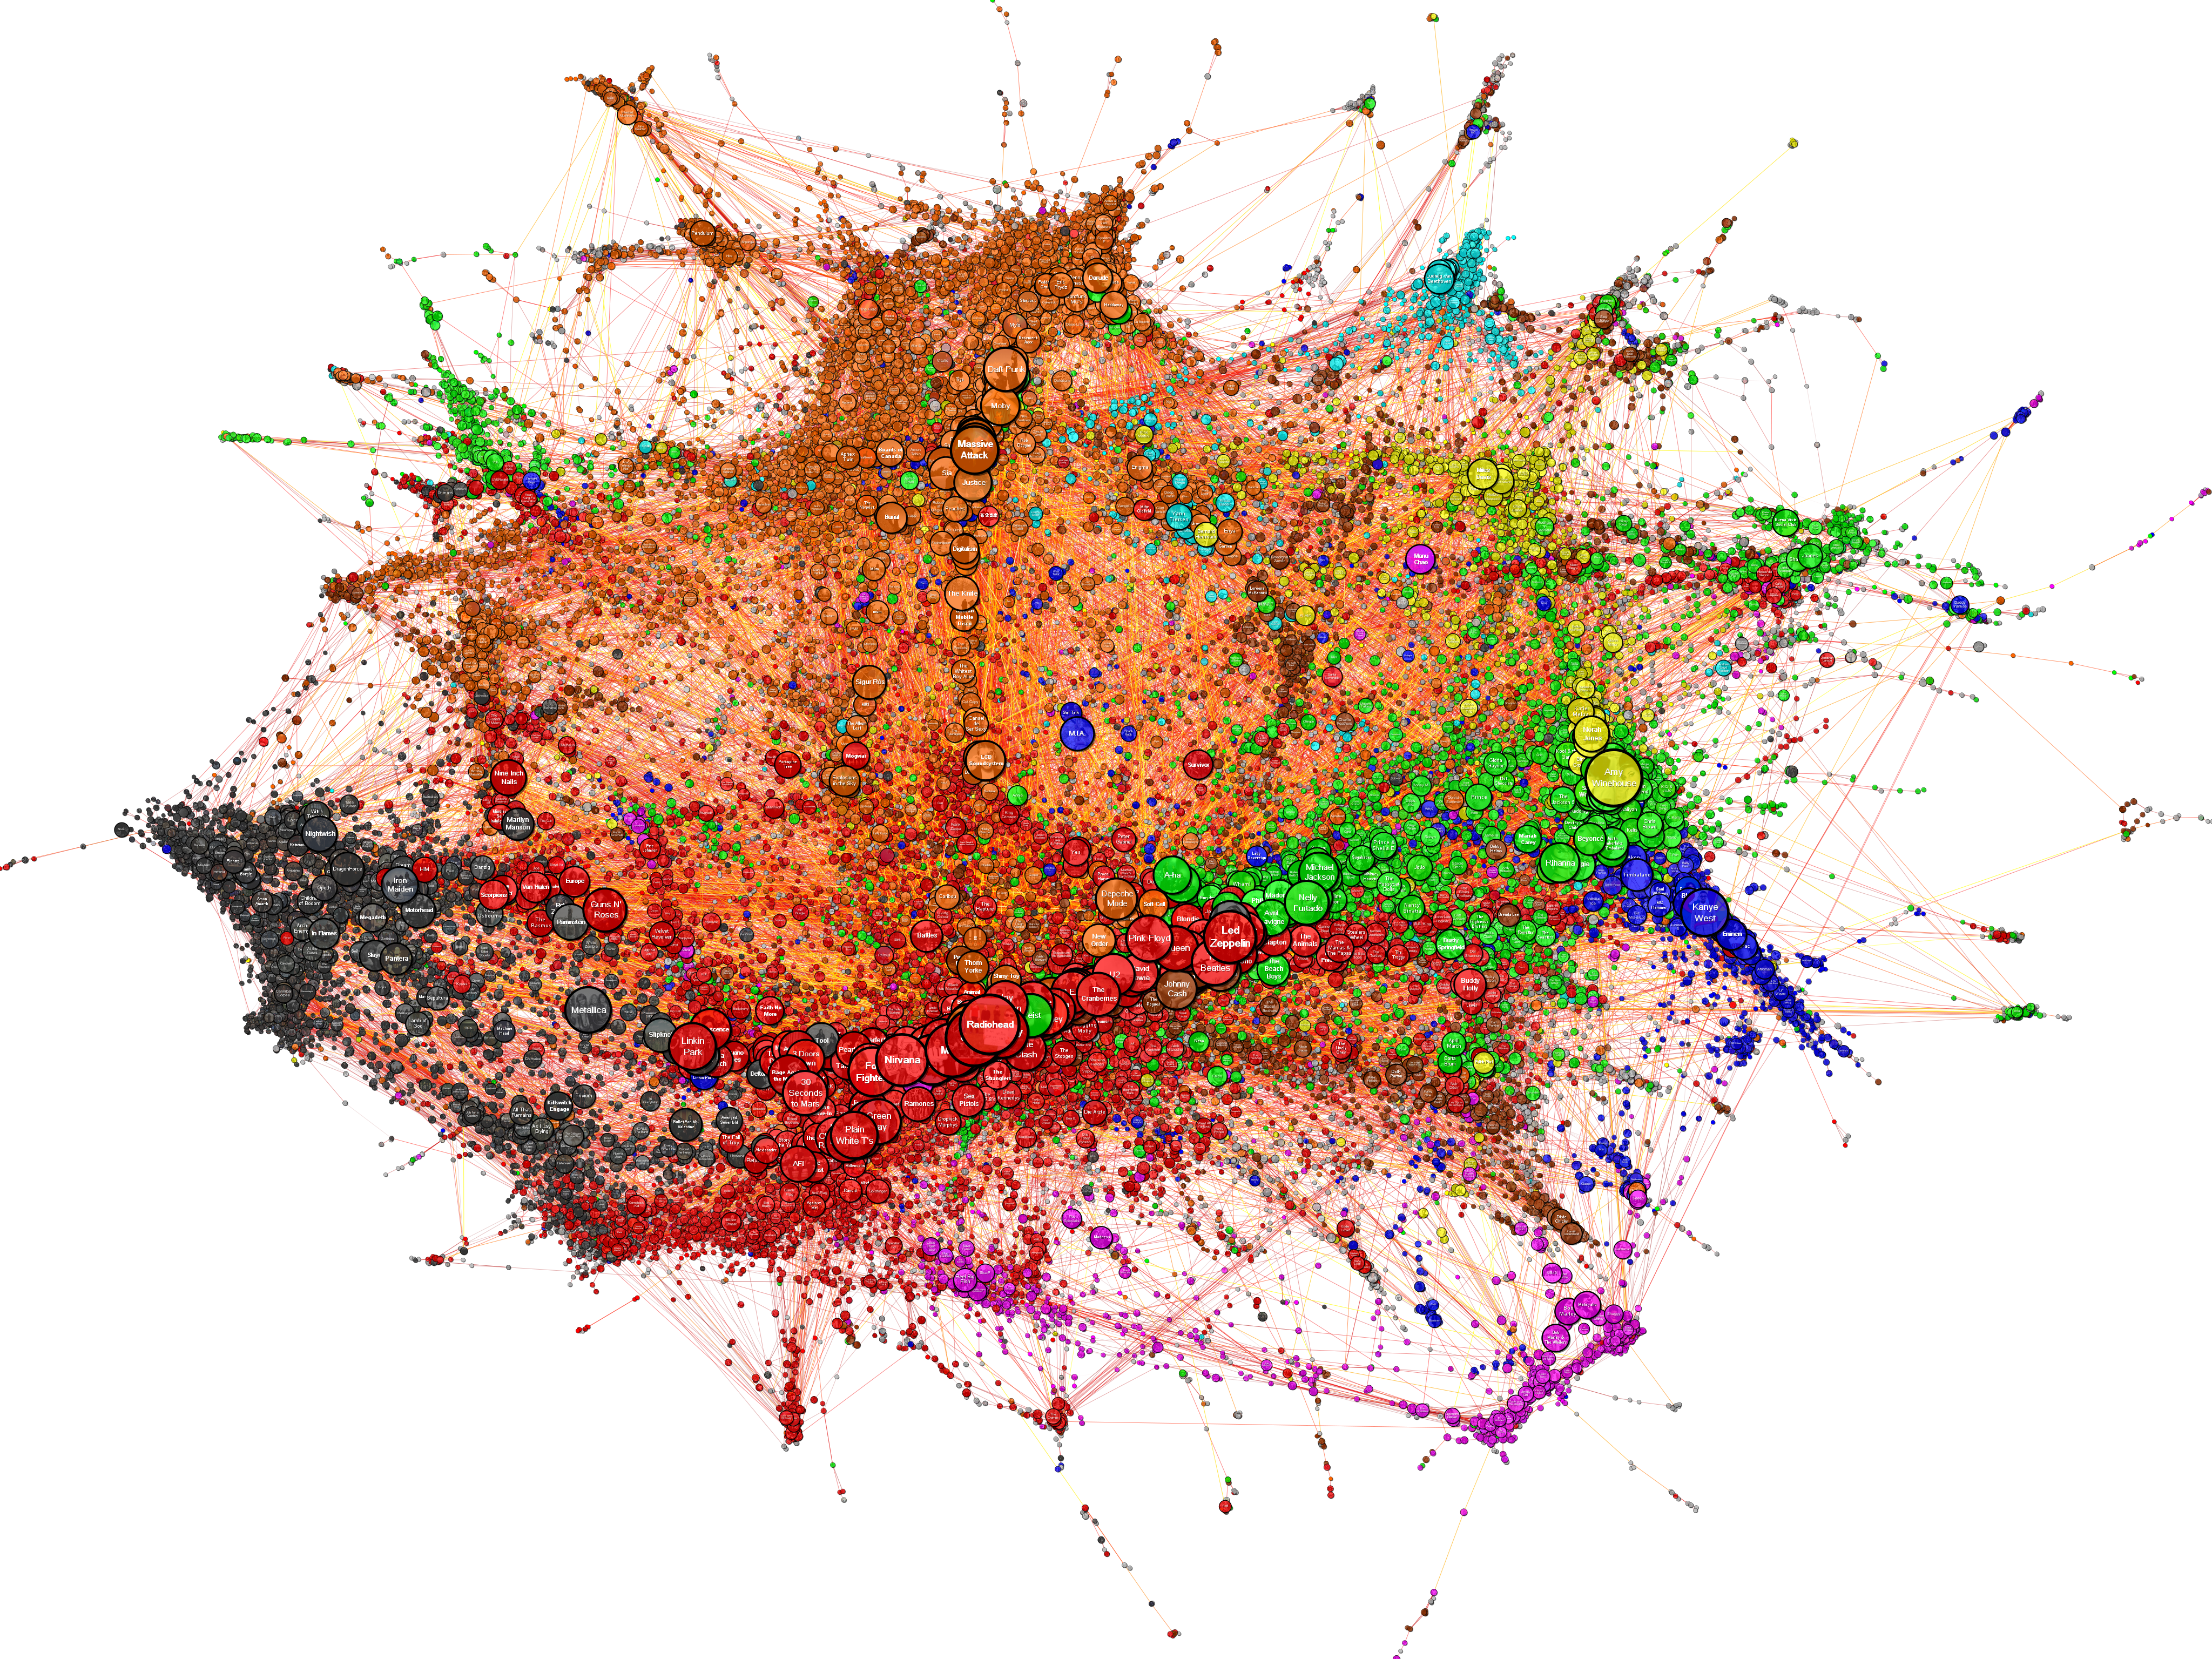
\includegraphics[width=\linewidth,height=0.8\textheight,keepaspectratio]{music}\\
\tiny Source: Last.fm's artist similarity network (\url{http://sixdegrees.hu/last.fm/index.html})
\end{frame}
%NOTE =============
%== The similarity is calculated on the basis of tags given to artists.
%== Rock is red, metal is dark grey, electronic is orange, hip-hop and rap is blue, jazz is yellow, reggae and ska is magenta, classical music is cyan, country, folk and world music is brown, pop is green. Light grey vertices are unclassified. See the technical details if you are interested in how the
%=================
%------------------------------------------------

\begin{frame}
\frametitle{\insertsection}
\framesubtitle{Example}
\centering
\includegraphics[width=\linewidth,height=0.8\textheight,keepaspectratio]{networks}\\
\tiny Source: N (nodes), L (links), <K> (average degree) \cite{Barabasi2016}
\end{frame}

%------------------------------------------------




%=======================================================
% `Social' Network Analysis and its origins
%=======================================================
\section{`Social' Network Analysis and its origins}
%------------------------------------------------

\bgroup
\setbeamercolor{background canvas}{bg = navyblue}
\begin{frame}[plain]{}
\begin{center}
\color{white}{\Huge\insertsection}
\end{center}
\end{frame}
\egroup

%------------------------------------------------

\begin{frame}
\frametitle{\insertsection}

{\color{blue}{Social Network Analysis}} is a perspective that encompasses theories, models, and applications that are expressed in terms of relations among social units (e.g.\ individuals, groups, communities, organisations, etc.)\\
\cite{Wassermann1994}

\end{frame}

%------------------------------------------------

\begin{frame}
\frametitle{\insertsection}

\centering
\includegraphics[width=0.8\linewidth,height=0.5\textheight,keepaspectratio]{scott}\\
\tiny Source: \cite{Scott2000}

\end{frame}

%NOTE =============
%==Attribute data relate to the attitudes, opinions, and behaviour of agents --- i.e. they are properties that belong to individuals and groups. We analyse this data with variable analysis.
%==Relational data are contacts, ties, and connections, etc. which relate one agent to the other --- they cannot be reduced to properties of individuals. We analyse these data with network analysis.
%==Ideational data describe the meanings, motives, definitions and typifications themselves. These include data that are subject to individual judgement or interpretation (e.g. sacred places). Typological analysis is a strategy for descriptive qualitative (or quantitative) data analysis whose goal is the development of a set of related but distinct categories within a phenomenon that discriminate across the phenomenon. -- development of ideal types or model cases
%==Despite their diversity these data are often collected together.
%=================

%------------------------------------------------

\begin{frame}
\frametitle{\insertsection}

\begin{itemize}
	\item Mathematics
	\item Anthropology
	\item Psychology
\end{itemize}

\end{frame}

%------------------------------------------------

\begin{frame}
\frametitle{\insertsection}

{\color{blue}{Mathematics}}: development of the mathematical notation ({\color{blue}{graph theory}}) to describe and identify solutions of relatively complex problems
	\begin{itemize}
	\item Euler's Konigsberg Bridge problem (1736)
	\item Markov-chain of probabilities
	\end{itemize}	

\end{frame}

%===
% Königsberg is the name for a former German city that is now Kaliningrad, Russia. 

%------------------------------------------------

\begin{frame}
\frametitle{\insertsection}

\centering
\includegraphics[width=\linewidth,height=0.7\textheight,keepaspectratio]{konigsberg1}\\
\tiny{Source: Euler and the seven bridges of Konigsberg [\url{http://eulerarchive.maa.org}]}
	
\begin{textblock*}{6cm}(8cm,2cm)
\includegraphics[width=2cm]{Euler}
\end{textblock*}

\end{frame}

%------------------------------------------------

\begin{frame}

\frametitle{\insertsection}
\centering
\includegraphics[width=\linewidth, frame]{poll1}

\end{frame}

%------------------------------------------------

\begin{frame}
\frametitle{\insertsection}

\centering
\includegraphics[width=\linewidth,height=0.7\textheight,keepaspectratio]{markov}\\
\tiny{Source: Markov-chain for weather forecasting [\url{www.americanscientist.org}]}
	
\end{frame}

%------------------------------------------------

\begin{frame}
\frametitle{\insertsection}

\begin{columns}[c]
\column{.45\textwidth} 
{\color{blue}{Anthropology}}
	\begin{itemize}
	\item 1950s: researchers of the Dept. of Social Anthropology at Manchester University examined the structure of community relations in tribal and villages societies
	\item 1960s-1970s: researchers at Harvard developed the mathematical component of social network analysis (e.g.\ network measures)
	\end{itemize}


\column{.45\textwidth}
\centering
\includegraphics[width=\linewidth]{granovetter}\\
\tiny Source: The strength of weak ties \cite{Granovetter1973}
\end{columns}

\end{frame}

%------------------------------------------------

\begin{frame}
\frametitle{\insertsection}

\begin{columns}[c]
\column{.45\textwidth} 
{\color{blue}{Psychology}}
         \begin{itemize}
	\item Gestalt studies in the 1920s on how mind works (organised patterns that structure thoughts and perceptions)
	\item Jacob Moreno and the development of {\color{blue}{sociometry}} (early 1930s)
	\item Kurt Lewin studied group behavior (individual-goal connections) (1930s)
	\item Fritz Heider's {\color{blue}{balance theory}} (1940s)
	\end{itemize}


\column{.45\textwidth}
\centering
\includegraphics[width=\linewidth]{moreno}\\
\tiny{Source: Sociogram of relationships between people \cite{Moreno1934}}
\end{columns}


\end{frame}

%NOTE =============
%== Moreno developed sociometry. He started asking people who their friends were and explored the ways in which their relations with others served as both limitations and opportunities for action and for their psychological behavior. Moreno invented the sociogram -- a diagram of points and lines used to represent relations among persons. Moreno used sociograms to identify social leaders and isolates, to uncover asymmetry and reciprocity in friendship choices, and to map chains of indirect connection.
%== Lewin studied group behavior, which he said was a function of conflicting social forces. Again, the field is seen as consisting of points connected by lines. The points are individuals, their goals, or their actions and the paths represent the interactional or causal sequences that connect them.
%== Heider worked in the area of social perception and attitudes. He developed what is known as balance theory. He said the mind seeks balance (an absence of tension) by trying to hold ideas that are not in conflict with one another. If A likes B, then A wants to like and dislike all the things that B likes and dislikes. If B dislikes C, then A wants to dislike C, but what if A and C are friends? There is a tension that must be resolved. One solution is to choose sides. A can dislike C.
%=================





%=======================================================
%	Branches of network analysis
%=======================================================
\section{Branches of network analysis}
%------------------------------------------------

\bgroup
\setbeamercolor{background canvas}{bg = navyblue}
\begin{frame}[plain]{}
\begin{center}
\color{white}{\Huge\insertsection}
\end{center}
\end{frame}
\egroup

%------------------------------------------------

\begin{frame}
\frametitle{\insertsection}


{\color{blue}{Descriptive network analysis}}\\ 
    \begin{itemize}
    \item An observed network is analysed by means of measures
    \item {\color{blue}{Network-level}} measures
    \item {\color{blue}{Node-level}} measures
    \end{itemize}

\bigskip
	
{\color{blue}{Modelling and inference of networks}}
    \begin{itemize}
    \item {\color{blue}{Mathematical models}}\\
    Based on `simple' probabilist rules to capture specific mechanisms (e.g.\ Erd\'os-R\'enyi networks, `the rich get richer')		
    \item {\color{blue}{Statistical models}}\\ 
    The observed network is considered as one of the possible realisation of a process -- a model that aims to fit to the observed data is specified (e.g.\ explanatory power of certain variables)
    \end{itemize}


\end{frame}

%------------------------------------------------

\begin{frame}
\frametitle{\insertsection}

Network Analysis is not a theory \textit{per se}, but it a methodological tool to support the development of theories \cite{Borgatti2011}

\begin{itemize}
    \item {\color{blue}{Network theory:}} mechanisms and processes that interact with network structures to produce certain outcomes for individuals, groups, and organisations (e.g.\ firms' performance, individuals' creativity)	
    
    \medskip
    
    \item {\color{blue}{Theory of networks:}} mechanisms and processes that explain why certain networks have certain structures (i.e.\ antecedents of network properties)
\end{itemize}

\end{frame}

%------------------------------------------------

\begin{frame}
\frametitle{\insertsection}

\centering
\includegraphics[width=8cm]{borgatti}\\
\tiny{Source: \cite{Borgatti2011}}
\end{frame}

%------------------------------------------------



%=======================================================
%	Key definitions
%=======================================================
\section{Key definitions}
%------------------------------------------------

\bgroup
\setbeamercolor{background canvas}{bg = navyblue}
\begin{frame}[plain]{}
\begin{center}
\color{white}{\Huge\insertsection}
\end{center}
\end{frame}
\egroup

%------------------------------------------------


\begin{frame}
\frametitle{\insertsection}
\framesubtitle{Undirected vs.\ directed and unweighted vs.\ weighted networks}

\begin{columns}[c]
\column{.45\textwidth}
\begin{itemize}
\item {\color{blue}{Tie directionality}}	
	\begin{itemize}
	\item<2-> {\color{blue}{Undirected networks}}: ties with no directionality (e.g.\ co-occurrence, alliances)
	\item<3-> {\color{blue}{Directed networks}}: ties with directionality (e.g.\ communication, transactions)
	\end{itemize}

\medskip

\item {\color{blue}{Tie value}}	
	\begin{itemize}
	\item<4-> {\color{blue}{Unweighted networks}}: ties with no weight (e.g.\ presence/absence)
	\item<5-> {\color{blue}{Weighted networks}}: ties with weights (e.g.\ frequency of interaction, amount of money associated with a transaction)
	\item<7-> {\color{blue}{Signed networks}}: positive and negative ties (e.g.\ loves vs.\ hates)
	\end{itemize}
\end{itemize}


\column{.45\textwidth}
\begin{minipage}[t]{\linewidth}

\centering

\includegraphics<1,2,4>[width=5cm]{base}

\includegraphics<3>[width=5cm]{directed}

\includegraphics<5>[width=5cm]{valued1}

\includegraphics<6>[width=5cm]{valued2}

\includegraphics<7>[width=5cm]{signed}

\end{minipage}

\end{columns}

\end{frame}

%------------------------------------------------

\begin{frame}
\frametitle{\insertsection}
\framesubtitle{Adjacency matrix}

\begin{columns}[c]
\column{.45\textwidth} 
	\begin{itemize}
		\item The (symmetric or asymmetric) matrix representing the connections among nodes is called {\color{blue}{adjacency matrix}}
		\item Relational data can be complemented with {\color{blue}{attributes}} of nodes (e.g.\ gender, education)
	\end{itemize}

\column{.45\textwidth}
\centering
\includegraphics[width=5cm]{base}
\[\mathbf{A} =\left(\begin{array}{@{}cccc@{}}
  								a_{11}&a_{12}&\cdots &a_{1N} \\
  								a_{21}&a_{22}&\cdots &a_{2N} \\
  								\vdots & \vdots & a_{ij} & \vdots\\
  								a_{N1}&a_{N2}&\cdots &a_{NN}
								\end{array}\right)\]

\end{columns}

\end{frame}

%------------------------------------------------

\begin{frame}
\frametitle{\insertsection}
\framesubtitle{Adjacency matrix: Undirected and unweighted network}

\begin{columns}[c]
\column{.45\textwidth} 
\centering
\includegraphics[width=5cm]{base}

\column{.45\textwidth}
\centering
\[\mathbf{A} =\left(\begin{array}{@{}ccccccc@{}}
0 & 1 & 1 & 0 & 0 & 0 & 0\\
1 & 0 & 1 & 0 & 1 & 0 & 0\\
1 & 1 & 0 & 1 & 1 & 0 & 0\\
0 & 0 & 1 & 0 & 0 & 0 & 0\\
0 & 1 & 1 & 0 & 0 & 1 & 1\\
0 & 0 & 0 & 0 & 1 & 0 & 0\\
0 & 0 & 0 & 0 & 1 & 0 & 0\\
\end{array}\right)\]

\end{columns}

\end{frame}

%------------------------------------------------

\begin{frame}
\frametitle{\insertsection}
\framesubtitle{Adjacency matrix: Undirected and unweighted network (exercise)}

\begin{columns}[c]
\column{.45\textwidth} 
\centering
\includegraphics[width=5cm]{adj_exercise}

\column{.45\textwidth}
\centering
What is the adjacency matrix\\
of this network?
\end{columns}

\end{frame}

%NOTE =============
%== 0 1 0 1 1
%== 1 0 0 1 1
%== 0 0 0 1 1
%== 1 1 1 0 0
%== 1 1 1 0 0
%=================

%------------------------------------------------

\begin{frame}
\frametitle{\insertsection}
\framesubtitle{Adjacency matrix: Directed and unweighted network}

\begin{columns}[c]
\column{.45\textwidth} 
\centering
\includegraphics<1>[width=5cm]{directed}

\column{.45\textwidth}
\centering
\[\mathbf{A} =\left(\begin{array}{@{}ccccccc@{}}
0 & 1 & 1 & 0 & 0 & 0 & 0\\
0 & 0 & 1 & 0 & 1 & 0 & 0\\
0 & 0 & 0 & 1 & 1 & 0 & 0\\
0 & 0 & 0 & 0 & 0 & 0 & 0\\
0 & 0 & 0 & 0 & 0 & 1 & 1\\
0 & 0 & 0 & 0 & 0 & 0 & 0\\
0 & 0 & 0 & 0 & 0 & 0 & 0\\
\end{array}\right)\]

\end{columns}

\end{frame}

%------------------------------------------------

\begin{frame}
\frametitle{\insertsection}
\framesubtitle{Adjacency matrix: Undirected and weighted network}

\begin{columns}[c]
\column{.45\textwidth} 
\centering
\includegraphics<1>[width=5cm]{valued1}

\column{.45\textwidth}
\centering
\[\mathbf{A} =\left(\begin{array}{@{}ccccccc@{}}
0 & 1.0 & 2.0 & 0.0 & 0.0 & 0 & 0\\
1 & 0.0 & 3.5 & 0.0 & 4.0 & 0 & 0\\
2 & 3.5 & 0.0 & 5.5 & 6.8 & 0 & 0\\
0 & 0.0 & 5.5 & 0.0 & 0.0 & 0 & 0\\
0 & 4.0 & 6.8 & 0.0 & 0.0 & 2 & 1\\
0 & 0.0 & 0.0 & 0.0 & 2.0 & 0 & 0\\
0 & 0.0 & 0.0 & 0.0 & 1.0 & 0 & 0\\
\end{array}\right)\]

\end{columns}

\end{frame}

%------------------------------------------------

\begin{frame}
\frametitle{\insertsection}
\framesubtitle{Adjacency matrix: Undirected and signed network}

\begin{columns}[c]
\column{.45\textwidth} 
\centering
\includegraphics<1>[width=5cm]{signed}

\column{.45\textwidth}
\centering
\[\mathbf{A} =\left(\begin{array}{@{}ccccccc@{}}
. & - & + & . & . & . & .\\
- & . & - & . & + & . & .\\
+ & - & . & - & + & . & .\\
. & . & - & . & . & . & .\\
. & + & + & . & . & - & +\\
. & . & . & . & - & . & .\\
. & . & . & . & + & . & .\\
\end{array}\right)\]

\end{columns}

\end{frame}

%------------------------------------------------

\begin{frame}
\frametitle{\insertsection}
\framesubtitle{Adjacency, dyads, and triads}

\begin{columns}[c]
\column{.45\textwidth} 
    \begin{itemize}
    \item<1-> Two nodes, $n_i$ and $n_j$ are called {\color{blue}{adjacent}} if an edge $e_k=(n_i, n_j)$ between them exists
    \item<2-> A {\color{blue}{dyad}} is a pair of nodes and the edge between them
    \item<3-> A {\color{blue}{triad}} is a set of three nodes and the edges between them
    \end{itemize}

\column{.45\textwidth}
\centering
\includegraphics<1>[width=5cm]{base}
\includegraphics<2>[width=5cm]{dyads}
\includegraphics<3>[width=5cm]{triads}
\end{columns}

\end{frame}

%------------------------------------------------

\begin{frame}
\frametitle{\insertsection}
\framesubtitle{Subgraphs}

\begin{columns}[c]
\column{.45\textwidth} 
	\begin{itemize}
		\item<1-> A {\color{blue}{subgraph}} of G is a graph $G_S(N_S, E_S)$ where $N_S \subseteq N$ and $E_S \subseteq E$
		\begin{itemize}
			\item<2-> Node-generated: $N_S \subseteq N$ and $E_S$ includes the lines linking $N_S$
			\item<3-> Line-generated: $E_S \subseteq E$ and $N_S$ includes all the nodes linked by $E_S$
		\end{itemize}
	\end{itemize}

\column{.45\textwidth}
\centering
\includegraphics<1>[width=5cm]{base}
\includegraphics<2>[width=5cm]{nodegen}
\includegraphics<3>[width=5cm]{linegen}
\end{columns}

\end{frame}

%------------------------------------------------

\begin{frame}
\frametitle{\insertsection}
\framesubtitle{Walks, trails, paths}

\begin{columns}[c]
\column{.45\textwidth} 
\begin{itemize}
	\item<1-> A {\color{blue}{walk}} is a sequence of nodes and lines in which each node is adjacent with the nodes following and preceding it in the sequence
	\item<2-> A {\color{blue}{trail}} is a walk in which all links are distinct, but nodes can be repeated
	\item<3-> A {\color{blue}{path}} is a walk in which all nodes and links are distinct
\end{itemize}

\column{.45\textwidth}
\centering
\includegraphics<1,2,3>[width=5cm]{base}

\only<1>{\scalebox{0.7}{$Walk=(n_1, n_3, n_2, n_1, n_3, n_4)$}}

\only<2>{\scalebox{0.7}{$Trail=(n_3, n_5, n_2, n_1, n_3, n_4)$}}

\only<3>{\scalebox{0.7}{$Path=(n_1, n_2, n_3, n_4)$}}

\end{columns}

\end{frame}

%------------------------------------------------

\begin{frame}
\frametitle{\insertsection}
\framesubtitle{Walks, trails, paths}

\begin{columns}[c]
\column{.45\textwidth} 
\begin{itemize}
	\item<1-> A {\color{blue}{closed walk}} is a walk that begins and ends with the same node
	\item<2-> A {\color{blue}{tour}} is a walk in which each link is used at least once
	\item<3-> A {\color{blue}{cycle}} is a closed walk of at least three nodes in which links are distinct
\end{itemize}

\column{.45\textwidth}
\centering
\includegraphics<1,2,3>[width=5cm]{base}

\only<1>{\scalebox{0.7}{$Closed Walk=(n_1, n_3, n_5, n_2, n_1)$}}

\only<2>{\scalebox{0.6}{$Tour=(n_1, n_2, n_5, n_7, n_5, n_6, n_5, n_3, n_4, n_3, n_3)$}}

\only<3>{\scalebox{0.7}{$Cycle=(n_1, n_3, n_5, n_2, n_1)$}}

\end{columns}

\end{frame}

%------------------------------------------------

\begin{frame}
\frametitle{\insertsection}
\framesubtitle{Geodesic distance}

\begin{columns}[c]
\column{.45\textwidth} 
\begin{itemize}
	\item The shortest path between two nodes in the network is called {\color{blue}{geodesic distance}} $d(n_i, n_j)$
	\item If a network is not connected, the geodesic distance is infinite in at least one pair of nodes
\end{itemize}

\column{.45\textwidth}
\centering
\only<1>{\includegraphics[width=5cm]{base}\\
$d(n_i, n_j)$}

\only<2>{\includegraphics[width=5cm]{geodesic1}\\
$d(1,4)=2$}

\only<3>{\includegraphics[width=5cm]{geodesic2}\\
$d(1,7)=3$}
\end{columns}

\end{frame}

%------------------------------------------------

\begin{frame}
\frametitle{\insertsection}
\framesubtitle{Bipartite graphs/two-mode networks}


\begin{columns}[c]
\column{.45\textwidth} 
\begin{itemize}
	\item A {\color{blue}{bipartite graph}} or two-mode network is a network where two subsets of nodes $(N_1, N_2)$ exist and the links are only between nodes of distinct subsets
	\item Examples: author-affiliation, actor-movie, firm-patent, R\&D projects and partners, etc.
	\item More than two partitions of nodes can exist: {\color{blue}{s-partite graph}} or {\color{blue}{s-mode}} network
\end{itemize}

\column{.45\textwidth}
\centering
\includegraphics[width=5cm]{bipartite}
\end{columns}

\end{frame}

%------------------------------------------------

\begin{frame}
\frametitle{\insertsection}
\framesubtitle{Multigraphs/multiplex networks}

\centering
\includegraphics[width=\linewidth, height=0.8\textheight,keepaspectratio]{soccer_3mode}\\
\tiny{Source: \url{www.nytimes.com/interactive/2014/06/20/sports/worldcup/how-world-cup-players-are-connected.html}}
	
\end{frame}
 

%------------------------------------------------

\begin{frame}
\frametitle{\insertsection}
\framesubtitle{Bipartite graphs vs.\ Hypergraphs}

\begin{itemize}
	\item In some networks, links can join {\color{blue}{more than two vertices}} (e.g.\ more than two authors on a publication)
	\item We can represent these with {\color{blue}{hypergraphs}}, where circles around groups of vertices are called {\color{blue}{hyperedges}}
\end{itemize}


\centering
\includegraphics[width = 0.8\textwidth]{hyper}\\
\tiny{Source: \cite{Newman2010}}

\end{frame}

%------------------------------------------------

\begin{frame}
\frametitle{\insertsection}
\framesubtitle{Multigraphs/multiplex networks} 

\begin{columns}[c]
\column{.45\textwidth} 
\begin{itemize}
	\item A {\color{blue}{multigraph}} or {\color{blue}{multiplex network}} is a network where nodes are linked by different sets of edges $(E_1, E_2, ... E_R)$
	\item Examples: "who do you seek advice on job" vs. "who is your friend"
\end{itemize}

\column{.45\textwidth}
\centering
\includegraphics[width=5cm]{multiplex}

\end{columns}

\end{frame}

%------------------------------------------------

\begin{frame}
\frametitle{\insertsection}
\framesubtitle{Multigraphs/multiplex networks}

\centering
\includegraphics[width=\linewidth,height=0.7\textheight,keepaspectratio]{multiplex_layers}\\
\tiny{Source: \cite{Kivela2014}}
	
\end{frame}

%------------------------------------------------

\begin{frame}
\frametitle{\insertsection}
\framesubtitle{Multigraphs/multiplex networks}

\centering
\includegraphics[width=\linewidth,height=0.7\textheight,keepaspectratio]{powell}\\	
\tiny{Source: Renaissance Florence \cite{Powell2012}}
	
\end{frame}

%------------------------------------------------

\begin{frame}
\frametitle{\insertsection}
\framesubtitle{Ego-network}

\begin{columns}[c]
\column{.45\textwidth} 
\begin{itemize}[<+->]
	\item The {\color{blue}{ego-network}} of a node $i$ is the set of nodes that are directly ($d(i,j)=1$) linked to $i$ (ego) and all the lines among these nodes
\end{itemize}

\column{.45\textwidth}
\centering
\includegraphics<1>[width=5cm]{base}
\includegraphics<2>[width=5cm]{egonet}

\end{columns}

\end{frame}

%------------------------------------------------

\begin{frame}
\frametitle{\insertsection}
\centering
\includegraphics[width=\linewidth, frame]{poll2}
\end{frame}

%------------------------------------------------

\begin{frame}
\frametitle{\insertsection}
\centering
\includegraphics[width=\linewidth, frame]{poll3}
\end{frame}

%------------------------------------------------

\begin{frame}
\frametitle{\insertsection}
\centering
\includegraphics[width=\linewidth, frame]{poll4}
\end{frame}

%------------------------------------------------







%%=======================================================
%	Next time ...
%%=======================================================
\section*{Next time ...}

%------------------------------------------------

\bgroup
\setbeamercolor{background canvas}{bg = navyblue}
\begin{frame}[plain]{}
\begin{center}
\color{white}{\Huge\insertsection}
\end{center}
\end{frame}
\egroup

%-----------------------------------

\begin{frame}
\frametitle{\insertsection}

\begin{itemize}
\item 	\textbf{Seminar: Network definition}
	\begin{itemize}
	\item Short intro to R
	\item Basic commands of the igraph package 
	\end{itemize}		
\medskip
\medskip
\item 	\textbf{Lecture: Network data collection}
	\begin{itemize}
	\item Main approaches to collect and sample network data 
	\item Network boundary specification problem
	\end{itemize}


\end{itemize}

\end{frame}

%------------------------------------------------

\begin{frame}
\frametitle{Assessment modes}

\textbf{Coursework}\\
\begin{itemize}
\item Groups up to 3 students
\item Report your group by Week 3: \href{https://bit.ly/2KLKCJ6}{\smash{https://bit.ly/2KLKCJ6}}
\item Small-scale network analysis project using novel or existing network data
\item {\color{orange}{Any topic!}}
\item Assessment modes:
	\begin{itemize}
	\item \textbf{Group Written Submission (GWS)} {\color{blue}{[30\% weighting]}}\\
		 Infographic poster (A1-size, PDF)
	\item \textbf{Group Presentation (GPN)} {\color{blue}{[20\% weighting]}}\\
	10-minute video recording presenting the infographic poster (GWS)
	\end{itemize}
\item Submission in Week 11 (see Canvas)
\item Marking criteria (see Canvas)
\end{itemize}

\bigskip

\centering
\includegraphics[width=\linewidth]{flow_chart_group_work}\\

\end{frame}

%------------------------------------------------

\begin{frame}
\frametitle{Extra - World Cup 2022 player-level network showing previous and current teammate relationships}
\centering
\includegraphics[width=\linewidth,height=0.7\textheight,keepaspectratio]{wc2022}\\
\tiny{Source: \url{https://nightingaledvs.com/fifa-world-cup-2022-the-network-edition/}}
\end{frame}

%=======================================================
%	Questions
%=======================================================
\bgroup
\setbeamercolor{background canvas}{bg = orange}
\begin{frame}[plain]{}
\begin{center}
\color{white}{\Huge Questions}
\end{center}
\end{frame}
\egroup








%=======================================================
%	References
%=======================================================
\begin{frame}[allowframebreaks]
\frametitle{References}
\tiny
\bibliographystyle{apalike}
\bibliography{library.bib}
%\bibliography{/Users/danielerotolo/Dropbox/References/bibtex_references/library.bib}
\end{frame}
%=======================================================


\end{document}